\documentclass[]{article}
\usepackage{ifpdf}

\synctex=1

\newcommand{\Title}{Perfect Epidemics}
\usepackage[british]{babel}
\newcommand{\Date}{\today}

%%%%%%%%%%%%%%%%%%%%%%%%%%%%%%%%
%% Various packages.
\usepackage{calc, xspace}
\usepackage{amsmath, amsthm, amsfonts, euscript}

%%%%%%%%%%%%%%%%%%%%%%%%%%%%%%%%
%% Bibtex
\usepackage[longnamesfirst]{natbib}
\setcitestyle{round}

%%%%%%%%%%%%%%%%%%%%%%%%%%%%%%%%
%% Font selection
\usepackage{times}
\usepackage[T1]{fontenc}
% \usepackage[utf8x]{inputenc}
% \usepackage{ccfonts,eulervm}
% \usepackage[expert,altbullet,seriftt]{lucidabr}

%%%%%%%%%%%%%%%%%%%%%%%%%%%%%%%%
%% Tracking queries (NB also loads colours!)
% \RequirePackage[no-comment]{WSKtracking}  %% Colour and Graphics
\usepackage{graphicx}
\graphicspath{{./image/}}
\RequirePackage{WSKtracking}  %% Colour and Graphics

\definecolor{linkcolor}{named}{Maroon}
\definecolor{citecolor}{named}{PineGreen}
%\definecolor{pagecolor}{named}{Maroon}
\definecolor{urlcolor}{named}{RoyalPurple}
\definecolor{okcolor}{named}{OliveGreen}
\definecolor{alertcolor}{named}{BrickRed}

\ifpdf
 \DeclareGraphicsExtensions{.png,.jpg}%
\else
 \DeclareGraphicsExtensions{.eps,.ps,.png,.jpg}%
\fi

%%%%%%%%%%%%%%%%%%%%%%%%%%%%%%%%
%% Page format and latex key display
%\usepackage{a4wide}
\usepackage[totalwidth=480pt,totalheight=680pt]{geometry}
% totalwidth  <=  8.26in
% totalheight <= 11.00in
%
\usepackage[notcite,color]{showkeys}

%%%%%%%%%%%%%%%%%%%%%%%%%%%%%%%%
%% Material for hyperref package.
 \usepackage[
 \ifpdf
   pdftex,
   pdfstartview=FitH,
   unicode,
 \fi
 ]{hyperref}
% \PrerenderUnicode{Π}
% Then use, eg, \texorpdfstring{$\Pi$}{Π} in section title.
 \hypersetup{
 pdfauthor={Stephen B. Connor and Wilfrid S. Kendall},
 pdftitle={\Title},
% pdfsubject={Coupling for Brownian motions augmented with local times},
 }
 \hypersetup{pdfstartview=FitH}
 \hypersetup{citecolor=citecolor}
 \hypersetup{linkcolor=linkcolor}
% \hypersetup{pagecolor=pagecolor}
 \hypersetup{urlcolor=urlcolor}
 \hypersetup{colorlinks=true}

%%%%%%%%%%%%%%%%%%%%%%%%%%%%%%%%
%% Mathematics
\RequirePackage{WSKmaths}
%
\newcommand{\Infections}{\mathcal{I}}
\newcommand{\SIR}{S-I-R\xspace}
\newcommand{\Removals}{\mathcal{R}}
\DeclareMathOperator{\trans}{trans}
  
%%%%%%%%%%%%%%%%%%%%%%%%%%%%%%%%
%% Document
 \begin{document}
 \TrackingPreamble

%%%%%%%%%%%%%%%%%%%%%%%%%%%%%%%%
%% Title page
 \title{\Title}
 \author{%
\href{http://maths.york.ac.uk/www/sbc502}{Stephen B. Connor}% 
\footnote{\href{mailto:stephen.connor@york.ac.uk}%
{\scriptsize stephen.connor@york.ac.uk}}
\ and
\href{http://warwick.ac.uk/wsk}{Wilfrid S. Kendall}%
\footnote{\href{mailto:w.s.kendall@warwick.ac.uk}%
{\scriptsize w.s.kendall@warwick.ac.uk}}
 \footnote{WSK supported by EPSRC Research Grant EP/K013939.}
}
 \date{\Date}
 \maketitle

% =========================================   
\begin{abstract}\noindent
\TBC{(abstract)}
\end{abstract}

\noindent
\textbf{Keywords and phrases:} \\
\textsc{
CFTP; 
graphical representation;
marked point process;
MCMC; 
Metropolis-Hastings sampler;
Poisson point process;
\SIR epidemic; 
spatial immigration-death process;
}

% =========================================   
 \section{Introduction}\label{sec:introduction}
\TBC{  Long-ago previous work, from which we can eventually build up a historical account (no particular need to look at this right now!):\\
work by Frank Ball and others on coupling for epidemics, also
   \cite{KendallSaunders-1983},
   \cite{Kendall-1998d},
   \cite{KendallThoennes-1999},
   \cite{KendallMoeller-2000},
   \cite{CaiKendall-2002}.
   \\
 Also consider use of immigration-death processes by \cite{Stephens-2000}.
 \\
 Contrast \cite{ConnorKendall-2014}, where the \CFTP algorithm was obtained by considering the modelled random process.
 In the present case we use a notion of ``algorithmic time'' to evolve the entire trajectory of the modelled random process.
 Refer to \citet{BanerjeeKendall-2015} for another example of this in a coupling context.
 \\
 \citet{GibsonRenshaw-1998,GibsonRenshaw-2001} use MCMC to make inferences about the parameters of infectivity \(\alpha\) and removal \(\beta\) conditional on observed removals.
 We have a less ambitious objective to start with (to make inferences about the actual pattern of infections conditional on \(\alpha\) and \(\beta\) as well as observed removals, 
 \emph{though later we may try to do more}),
 but we seek a perfect simulation method.
}
%

The aim of this paper is to show how to conduct a perfect simulation of an \SIR epidemic, 
conditional on a given infection rate of \(\alpha\) per ordered pair of infected and susceptible individuals and a given removal rate of \(\beta\) per infected individual, 
and also conditioned on observation of the removals, presuming that all individuals are eventually infected and then removed from the population.%
\NB[WSK2]{Need to consider partial epidemics too, in which not all individuals are infected (and we may not know the true population size!}
Thus we seek to sample perfectly from the conditional distribution of infection incidents.

\TBC{
Structure of paper:\\
Section \ref{sec:introduction}: this introduction.\\
Section \ref{sec:SIR}: construction of \SIR epidemic using Poisson point processes to supply streams of potential incidents .\\
Section \ref{sec:algorithmic}: introduction to algorithmic time and simulation of the \SIR trajectory in algorithmic time.\\
Section \ref{sec:restrictions}: restrictions, conditioning and a modified construction.\\
Section \ref{sec:cftp}: monotonicity and \CFTP. \\
Section \ref{sec:examples}: simulations, fitting data.\\
Section \ref{sec:conclusion}: discussion and extensions.
\\
Presently this paper is drafted in a verbose, repetitive and often imprecise way; 
the purpose is to map out the general flow of the argument leading to perfect simulation of \SIR epidemics given complete observation of the removals.
}

% =========================================   
 \section{Poisson processes and \SIR epidemics}\label{sec:SIR}
% Use Poisson streams of potential incidents to generate S-I-R processes.
%
We begin by describing how to build \SIR epidemics using Poisson streams of potential incidents.

Suppose that the total population comprises \(n\) individuals.
Using the terminology of interacting particle systems (see for example \citealp[Section III.6]{Liggett-1985}), an unconditioned \SIR epidemic can be realized using a \emph{graphical representation}.
As a simple example, the evolution of an \SIR epidemic for this population of \(n\) individuals can be visualized using a set of \(n\) time-lines: 
one copy of the process time-axis \([0,\infty)\) for each individual in the population.
 Potential infection and removal incidents can be simulated by using independent Poisson streams of the different kinds of potential incidents, namely:
   \begin{enumerate}
    \item by using \(n\) independent Poisson processes of potential removals 
    (one Poisson \((\beta\)) process per time-line of individual);
    \item and by using \(\tbinom{n}{2}\) independent Poisson processes of potential infections 
    (one Poisson (\(\alpha\)) process per unordered pair of time-lines of two individuals, producing a stream of potentially infectious contacts).
   \end{enumerate}
 These streams of potential infection and removal incidents allow us to simulate \SIR epidemics from all possible sets of initial conditions simultaneously,%
\NB[WSK2]{Note possibility of omnithermal simulation?}
 using the two following natural rules: 
 potential removal incidents are realized as actual removals if and only if the corresponding individual is actually infected just before the incident,
 and in this case the individual changes from infected to removed at the time of the incident;
 potential infections are realized as actual infections if one of the two corresponding individuals is actually infected just before the incident
 and the other is susceptible, and in this case the susceptible individual changes from susceptible to infected at the time of the incident.
 In theory we could carry out such simulations running over the complete process time-scale \([0,\infty)\),
 though in practice we will restrict attention to some bounded time-interval \([0,T]\).%
\NB[WSK2]{Hence $T$, the length of time over which we are simulating the (eventually removal-conditioned) \SIR epidemic, recurs throughout this exposition!}

 To enable precise statements about transitions, we adopt the convention that the trajectories of the states of individuals all possess the ``c\`adl\`ag'' property. 
 This is to say, the trajectories are continuous from the right (``continue \`a droite'') and have limits from the left (``limites \`a gauche'').
 
 The above construction is the simplest graphical representation of an SIR epidemic.
 For purposes of perfect simulation we will need to consider a slightly more complicated variant;
 however for the purposes of exposition we first make some remarks about the simpler case.
 
 % =========================================   
 \section{Algorithmic time and simulation of stochastic dynamics}\label{sec:algorithmic}
% Constructing S-I-R epidemic trajectories using a trajectory-valued process driven by spatial immigration-death processes.
%
 We can realize the Poisson streams of potential incidents using \(n+\tbinom{n}{2}\) independent stationary spatial immigration-death processes, using an ``algorithmic time'' parameter \(\tau\in\Reals\).
 The spatial parameter \(t\in[0,\infty)\) of the immigration-death processes actually plays the part of the ``process time''.
 Running in algorithmic time \(\tau\), potential removal incidents for any given individual are introduced at algorithmic-time-rate \(\beta\) per unit of process time \(t\), 
 and specific removal incidents then die at unit algorithmic-time-rate per incident;
 potential infection incidents for any given pair of individuals are introduced at algorithmic-time-rate \(\alpha\) per unit of process time \(t\), and die at unit algorithmic-time-rate per incident.
 The spatial immigration-death processes being stationary, the spatial patterns formed by these immigration-death processes at any specific algorithmic time \(\tau\) then constitute
 independent Poisson streams of potential incidents (viewed in process time) as required by the graphical representation described in the first step above.
 Thus at a given algorithmic time \(\tau\) the pattern of potential infections and potential removals can be used to construct an entire trajectory of an \SIR epidemic evolving in process time.
 One can visualize algorithmic time as running orthogonal to the process time axis \([0,\infty)\).
 (Compare the use of algorithmic time to construct a simple but efficient non-Markovian coupling in \citealp{BanerjeeKendall-2015}.)

By construction, this trajectory-valued Markov chain running in algorithmic time has the \SIR epidemic as invariant distribution.
Renewal-theoretic arguments using small-set theory can show that the Markov chain converges to the \SIR epidemic as a unique statistical equilibrium.%
\NB[WSK2]{Give details about the renewal-theoretic arguments using small-set theory showing that the free Markov chain converges to a unique statistical equilibrium}
So this allows us to simulate the evolution in algorithmic time of simultaneous coupled realizations of \SIR epidemics from all possible sets of initial conditions.
 We will say that the stochastic dynamics of a given realization is that of the \emph{free} Markov chain.
  We will seek coupling methods which are useful to analyze the process \((X, F(X))\), 
where \(F\) is a given measurable function of an \SIR-realization-valued Markov chain \(X\). 
This is somewhat related to an ongoing programme investigating immersion coupling for nilpotent diffusions (for recent overviews, see \citealp{Kendall-2009d,Kendall-2013a}).
 

 \begin{thm}\label{thm:SIR-epidemic-1}
 Suppose \(\widetilde{S}_t\), \(\widetilde{I}_t\), \(\widetilde{R}_t\) measure the susceptibles, infectives, and removals 
 arising at time \(\tau\) in stochastic equilibrium for the algorithmic-time process described above.
 If the algorithmic-time process is in equilibrium at time \(\tau\), then the trajectory \((\widetilde{S}, \widetilde{I}, \widetilde{R})\), viewed in process time, forms an \SIR epidemic.
\end{thm}
\begin{proof}[Sketch proof]
 Show that the process \((\widetilde{S}, \widetilde{I}, \widetilde{R})\) solves the relevant martingale problem in process time when sampled in equilibrium in algorithmic time,  
 citing results on the well-posedness of the martingale problem from \citet{StroockVaradhan-1979}.%
 \NB[WSK1]{Need to complete the statement and proof of Theorem \ref{thm:SIR-epidemic-1}.}
\end{proof}


 
% =========================================   
\section{Restrictions, conditioning and a modified
  construction}\label{sec:restrictions}
% Implementing conditioning on removals by fixing actual times of
% removal for the dynamic process evolving in algorithmic time.
%
The independent immigration-death processes, described in Section
\ref{sec:algorithmic} above, are reversible in time, and the resulting
evolution of the \SIR trajectory realization therefore inherits the
time-reversibility property.  This facilitates the task of sampling
from \emph{conditioned} realizations: suppose that our target is to
draw from the \SIR distribution with trajectory conditioned to lie in
a fixed subset \(A\) of the space of possible trajectories.  Subject
to reducibility considerations, we can obtain this conditional
distribution as the statistical equilibrium of a Metropolis-Hastings
sampler: view each birth or death of a potential incident as a
proposal, to be accepted if the trajectory remains in \(A\) and
rejected otherwise.


% \TBC{ Conditioning on removal times
% \\
% Our objective is to obtain a Markov chain whose equilibrium
% distribution is the conditional distribution of the \SIR epidemic
% conditional on all individuals being infected, and all removals
% being observed to occur at exactly specified times.  (Variations on
% this may be feasible, at the price of additional complexity.)  We
% use a fundamental fact about reversible Markov chains: restriction
% of state-space leads to equilibria which are conditional
% distributions.  One simply needs to check that the Markov chain in
% the restricted state-space is irreducible and positive-recurrent.  }
 
This gives rise to a modified Markov chain taking values in trajectory
space; so long as the modified Markov chain is irreducible%
\NB[WSK2]{Better to talk about Harris property rather than
  irreducibility?!}  then it can be shown that the modified chain will
automatically converge in distribution to an equilibrium which is the
target conditional distribution.  We say this modified Markov chain is
the \emph{constrained} Markov chain.

If we wish to condition on actual times of removal then this
convergence result is not applicable in the form prescribed above.
Suppose we consider the case when there is just one initial infective
and we condition on \(n-1\) specified times of removal (almost surely
there then will be \(n-1\) such times).  The resulting subset \(A\) of
trajectory space produces a \emph{reducible} constrained Markov chain,
since it is not possible to alter which individual is removed at the
first removal time, \emph{et cetera}.  This could perhaps be overcome
using symmetry considerations; however it also appears to be difficult
to discover any monotonicity structure, given the exchangeability of
the \(n\) individuals involved.  These considerations motivate the
introduction of a variant free Markov chain (and consequently of a
variant constrained Markov chain).

The first component of the variation is to observe that we can require
that the initial configuration of \(R_0\) removed, \(I_0\) infected,
and \(S_0\) susceptible individuals must be arranged in index order,
with individuals \(1, \ldots, R_0\) being initially removed, \(R_0+1,
..., R_0+I_0\) initially infected, and \(R_0+I_0+1, \ldots,
R_0+I_0+S_0=n\) initially susceptible.  With no loss of generality
(since removed individuals have no further effect on the stochastic
evolution of the trajectory), in practice one could set \(R_0=0\).

We now change the dynamics of the algorithmic time evolution so that
removals, infectives and susceptibles continue for all algorithmic
time \(\tau\) to be given by three contiguous ranges partitioning
\(\{1, \ldots, n\}\): we obtain this by working with the following
Poisson streams of potential incidents.  Potential removals applying
to an individual \(m\) form a Poisson (\(m\beta\)) point process of
incidents in algorithmic time, independently marked by draws from a
Uniform (\(\{1, \ldots, m\}\)) distribution, while potential
infections applying to an individual \(m\) form a Poisson (\(m
(n-m)\alpha\)) point process of incidents in algorithmic time, again
independently marked by draws from a Uniform (\(\{1, \ldots, m\}\))
distribution.  All these marked Poisson point processes are
independent of each other.

A potential removal or infection at process time \(t\) for the
\(m^\text{th}\) individual only become actual if (a) individual \(m\)
is currently (at time \(t-\)) the infected individual of highest
index, and (b) the corresponding mark exceeds \(R_{t-}\). In that
case:
\begin{itemize}
\item for a removal, individual \(R_{t-}+1\) is switched from
  infective to removed at time \(t\), so \(R_t=R_{t-}+1\),
  \(I_t=I_{t-}-1\); %
\item for an infection, individual \(m+1\) is switched from
  susceptible to infected at time \(t\), so \(I_t=I_{t-}+1\),
  \(S_t=S_{t-}-1\).
\end{itemize}
% On the other hand, a potential infection at process time \(t\) for
% the \(m^\text{th}\) individual only becomes actual if (a) individual
% \(m\) is currently (at time \(t-\)) the infected individual of
% highest index, (b) the corresponding mark exceeds \(R_{t-}\).  In
% that case, individual \(m+1\) is switched from susceptible to
% infected at time \(t\), so \(I_t=I_{t-}+1\), \(S_t=S_{t-}-1\).
For both potential removal and infection incidents, the Uniform
(\(\{1, \ldots, m\}\)) mark is used to thin out the number of proposed
incidents to match the correct rate for the \SIR
epidemic.\xNB[WSK2]{Need to remark somewhere that all our random
  processes have \emph{c\`adl\`ag} trajectories.}

 
It follows immediately (by an argument using induction over the
time-ordered set of potential incidents) that at process time \(t\)
the individuals \(1, \ldots, R_t\) are removed, \(R_t+1, ...,
R_t+I_t\) are infected, and \(R_t+I_t+1, \ldots, R_t+I_t+S_t=n\) are
susceptible.

The second component of the variation is to separate out the updates
of potential removals and potential infections in algorithmic time.
This is directly analogous to using a systematic scan for the
heat-bath dynamics for the Ising model.%
\NB[WSK2]{Supply appropriate reference to systematic scans for the
  Ising model.}  For simplicity suppose that we are simulating over a
process time interval \([0,T]\) for some fixed deterministic time
\(T\).  Over a period \([2(k-1)T, 2kT)\) of algorithmic time we take
the following steps:%
\xNB[SBC]{Changed time period from $[2(m-1)T, 2mT)$ to $[2(k-1)T,
  2kT)$, so as to reduce potential for confusion caused by using $m$
  to enumerate timelines.}  \NB[WSK2]{Here we update using a vertical
  line moving forwards (for removals) then backwards (for infections)
  in process time, as opposed to the original TV-scan.}
\begin{enumerate}
\item Over the algorithmic time interval \([2(k-1)T, (2k-1)T)\),%
  \NB[WSK2]{No need to worry about whether a potential removal occurs
    exactly at time $(2k-1)T$! Almost surely this will never happen.}
  we re-sample all the potential removals as follows: create a new
  sample of potential removals over process time interval \([0,T]\),
  by algorithmic time \(2(k-1)T+t\) (for \(0\leq t<T\)) replace old
  potential removal incidents in process time interval \([0,t]\) by
  the corresponding new potential removal incidents in process time
  interval \([0,t]\).  (So almost surely by algorithmic time
  \((2k-1)T\) all old potential removal incidents will have been
  replaced by new potential removal incidents.)
  % \item Exactly at time \((m-1)T\) we re-sample the uniform marks
  %   corresponding to the various removal incidents.  (This step will
  %   prove to be crucial if we are to ensure that the result of
  %   restricting actual realized removals to specific nominated times
  %   still leads to an irreducible Markov chain.)
\item Over the algorithmic time interval \([(2k-1)T, 2kT)\),%
  \NB[WSK2]{No need to worry about whether a potential infection
    occurs exactly at time $2kT$! Almost surely this will never
    happen.}  we re-sample all the potential infections as follows:
  create a new sample of potential infections over process time
  interval \([0,T]\), by algorithmic time \((2k-1)T+t\) (for \(0\leq
  t< T\)) replace old potential infection incidents in process time
  interval \([T-t,T]\) by the corresponding new potential infection
  incidents in process time interval \([T-t,T]\).  (So almost surely
  by algorithmic time \(2kT\) all old potential infection incidents
  will have been replaced by new potential infection incidents.)
\end{enumerate}

A dynamic reversibility argument confirms that the time-inhomogeneous
Markov chain resulting from this modified construction still has the
\SIR epidemic as invariant distribution, and further arguments assure
us that this is the unique equilibrium distribution to which the chain
converges in distribution.%
\NB[WSK2]{Add details about the dynamic reversibility argument for the
  specified time-inhomogeneous Markov chain.}
\begin{thm}\label{thm:SIR-epidemic-2}
  Suppose \({S}_t\), \({I}_t\), \({R}_t\) measure the susceptibles,
  infectives, and removals arising at time \(\tau\) in stochastic
  equilibrium for the algorithmic-time process given by the modified
  construction described above.  The process \(({S}, {I}, {R})\),
  viewed in process time, forms an \SIR epidemic in equilibrium and
  more generally converges to this \SIR epidemic in distribution as
  algorithmic time tends to infinity.
\end{thm}
\begin{proof}[Sketch proof]
  Verify detailed (perhaps dynamic) balance is satisfied.  Show that
  the process \(({S}, {I}, {R})\) solves the relevant martingale
  problem in process time when sampled in equilibrium in algorithmic
  time, citing results on the well-posedness of the martingale problem
  from \citet{StroockVaradhan-1979}.%
  \NB[WSK1]{Need to complete the statement and proof of Theorem
    \ref{thm:SIR-epidemic-2}.}  Establish convergence to equilibrium.
\end{proof}


% \TBC{ The Poisson (\((x(n-x)\alpha\)) and Poisson (\(\beta\))
% patterns of marked incidents evolve in ``algorithmic time'' (one
% might think of this as ``orthogonal'' to ``process time'': ``process
% time'' runs along the time-line axis).  In one possible variant,
% they evolve in continuous algorithmic time as independent "spatial"
% (dimension \(d=1\)) immigration-death processes with unit death
% rates, and with immigration rates per unit time being \(\alpha\) and
% \(\beta\) respectively.  In another, they evolve in discrete
% algorithmic time, alternately replacing all potential removal
% incidents and all potential infection incidents.  In this second
% variant it is useful to track down the continuous process time axis,
% treating potential incidents ``pixel by pixel''.
% \\
% Reversibility
% \\
% In the first case (continuous algorithmic time), reversibility
% follows rather directly from reversibility of spatial
% immigration-death processes, and Theorem \ref{thm:SIR-epidemic-1} in
% Section \ref{sec:SIR}, that a realization of the SIR epidemic can be
% achieved as a measurable function of the Poisson equilibrium.
% \\
% In the second case, one has to use notions of dynamic reversibility.
% }



Suppose the state-space is restricted by fixing all \(n\) observed
removal times as \(0<\rho_1<\rho_2<\ldots<\rho_n\).  The resulting
restrictions on the Markov chain in algorithmic time are as follows:%
\NB[WSK1]{Check the list of relevant restrictions on the Markov chain
  in algorithmic time.}
\begin{enumerate}
\item Proposals to introduce potential removals (other than
  conditioned removals) are refused if they would result in the
  introduction of new realized removals (equivalently, the
  introduction of potential removals occurring on infected parts of
  time-lines is always refused).
\item Proposals to delete potential removals are refused only if the
  removal in question is realized (equivalently, none of the observed
  removals constrained by conditioning can ever be removed).
  % \item Proposals to change the marks of potential removals are
  %   refused if they would result in the introduction of new actual
  %   removals.
  % \item Proposals to change the marks of actual (hence conditioned)
  %   removals are refused if they would result in there not being an
  %   observed removal at the relevant time.
\item Proposals to introduce potential infections are refused if they
  would then be realized and lead directly or indirectly to infection
  of a time-line before a potential, unrealized, removal.
\item Proposals to delete realized infections are refused if they
  would result in the epidemic not infecting the entire population.
\item[] If a proposal to remove a realized infection is refused, then
  we say that the retained infection is \emph{perpetuated}.
  % Note that perpetuated infections must therefore previously (in
  % algorithmic time) be actual infections.
\end{enumerate}

Because we have conditioned on all observed removal times, the process
of realized removals \(\{R_t:t\geq0\}\) can now be treated as
deterministic.
% If the removal of individual \(m\) is conditioned to occur at time
% \(t=\rho_m\) (thus \(R_t=m\)) then the associated Uniform (\(\{m,
% \ldots, n\}\)) mark \(\mu_m\) must also be conditioned to be no
% greater than \(R_{t-}+I_{t-}=m+I_{t-}-1\).
% % ,
% % with conditional distribution Uniform (\(\{m, \ldots,
% % m+I_{t-}-1\}\)).
% Thus the mark of a conditioned removal serves to define a threshold
% for the number of infectives, which must be exceeded at the time of
% removal.  Actual removal times being subject to conditioning, w
Potential removals are thinned using their associated marks, so the
(time-varying) rate of introduction of potential removals arising from
individual \(m\) at time \(t\) is given by \((m -R_t)\beta\): recall
that this removal will be realized (and will result in the removal of
individual $R_{t-}+1$) if and only if individual $m$ is the
highest-indexed infected individual at the relevant time, so that the
overall removal rate will be \(I_t \beta\) as required.%
\NB[WSK2]{I worry that there may be confusion between (a) the rates of
  introduction of various incidents in algorithmic time, and (b) the
  rates of introduction of various incidents in process time. Vary
  nomenclature?}
% These potential removals will be influential on the algorithmic-time
% evolution of the epidemic only if they occur on the un-removed
% portion of a time-line \(m\).
In order that the conditioning on observed removals be respected, the
introduction of a removal must be forbidden if it will immediately be
realized as a removal not specified by the conditioning.%
\NB[WSK2]{Repetition of need to forbid introduction of potential
  removals that destroy conditioning.}
 
Similarly potential infections are thinned using their associated
marks: consider a potential infection originating from individual
\(m\) at time \(t\) with Uniform(\(\{1, \ldots, m\}\)) mark.  This
potential infection is censored if the mark does not exceed \(R_t\).
Thus the (time-varying) rate of introduction of potential infections
arising from individual \(m\) at time \(t\) is given by
\((m-R_t)(n-m)\alpha\); recall that this infection will be realized if
and only if the individual concerned is the highest-indexed infected
individual at the relevant time, so that the overall infection rate
will be \(I_t S_t \alpha\) as required.  Again, the realization of a
potential infection must be forbidden if it leads to a removal not
specified by the conditioning.  Moreover the removal of a realized
infection (in the course of algorithmic time as specified above) must
be forbidden if thereby one would fail to produce a complete epidemic
with removals as specified by the conditioning.
% , and the mark conditional on removals is Uniform (\(\{R_t+1,
% \ldots, m\}\)).


Figure \ref{fig:graphical} illustrates this construction.
\begin{Figure}
  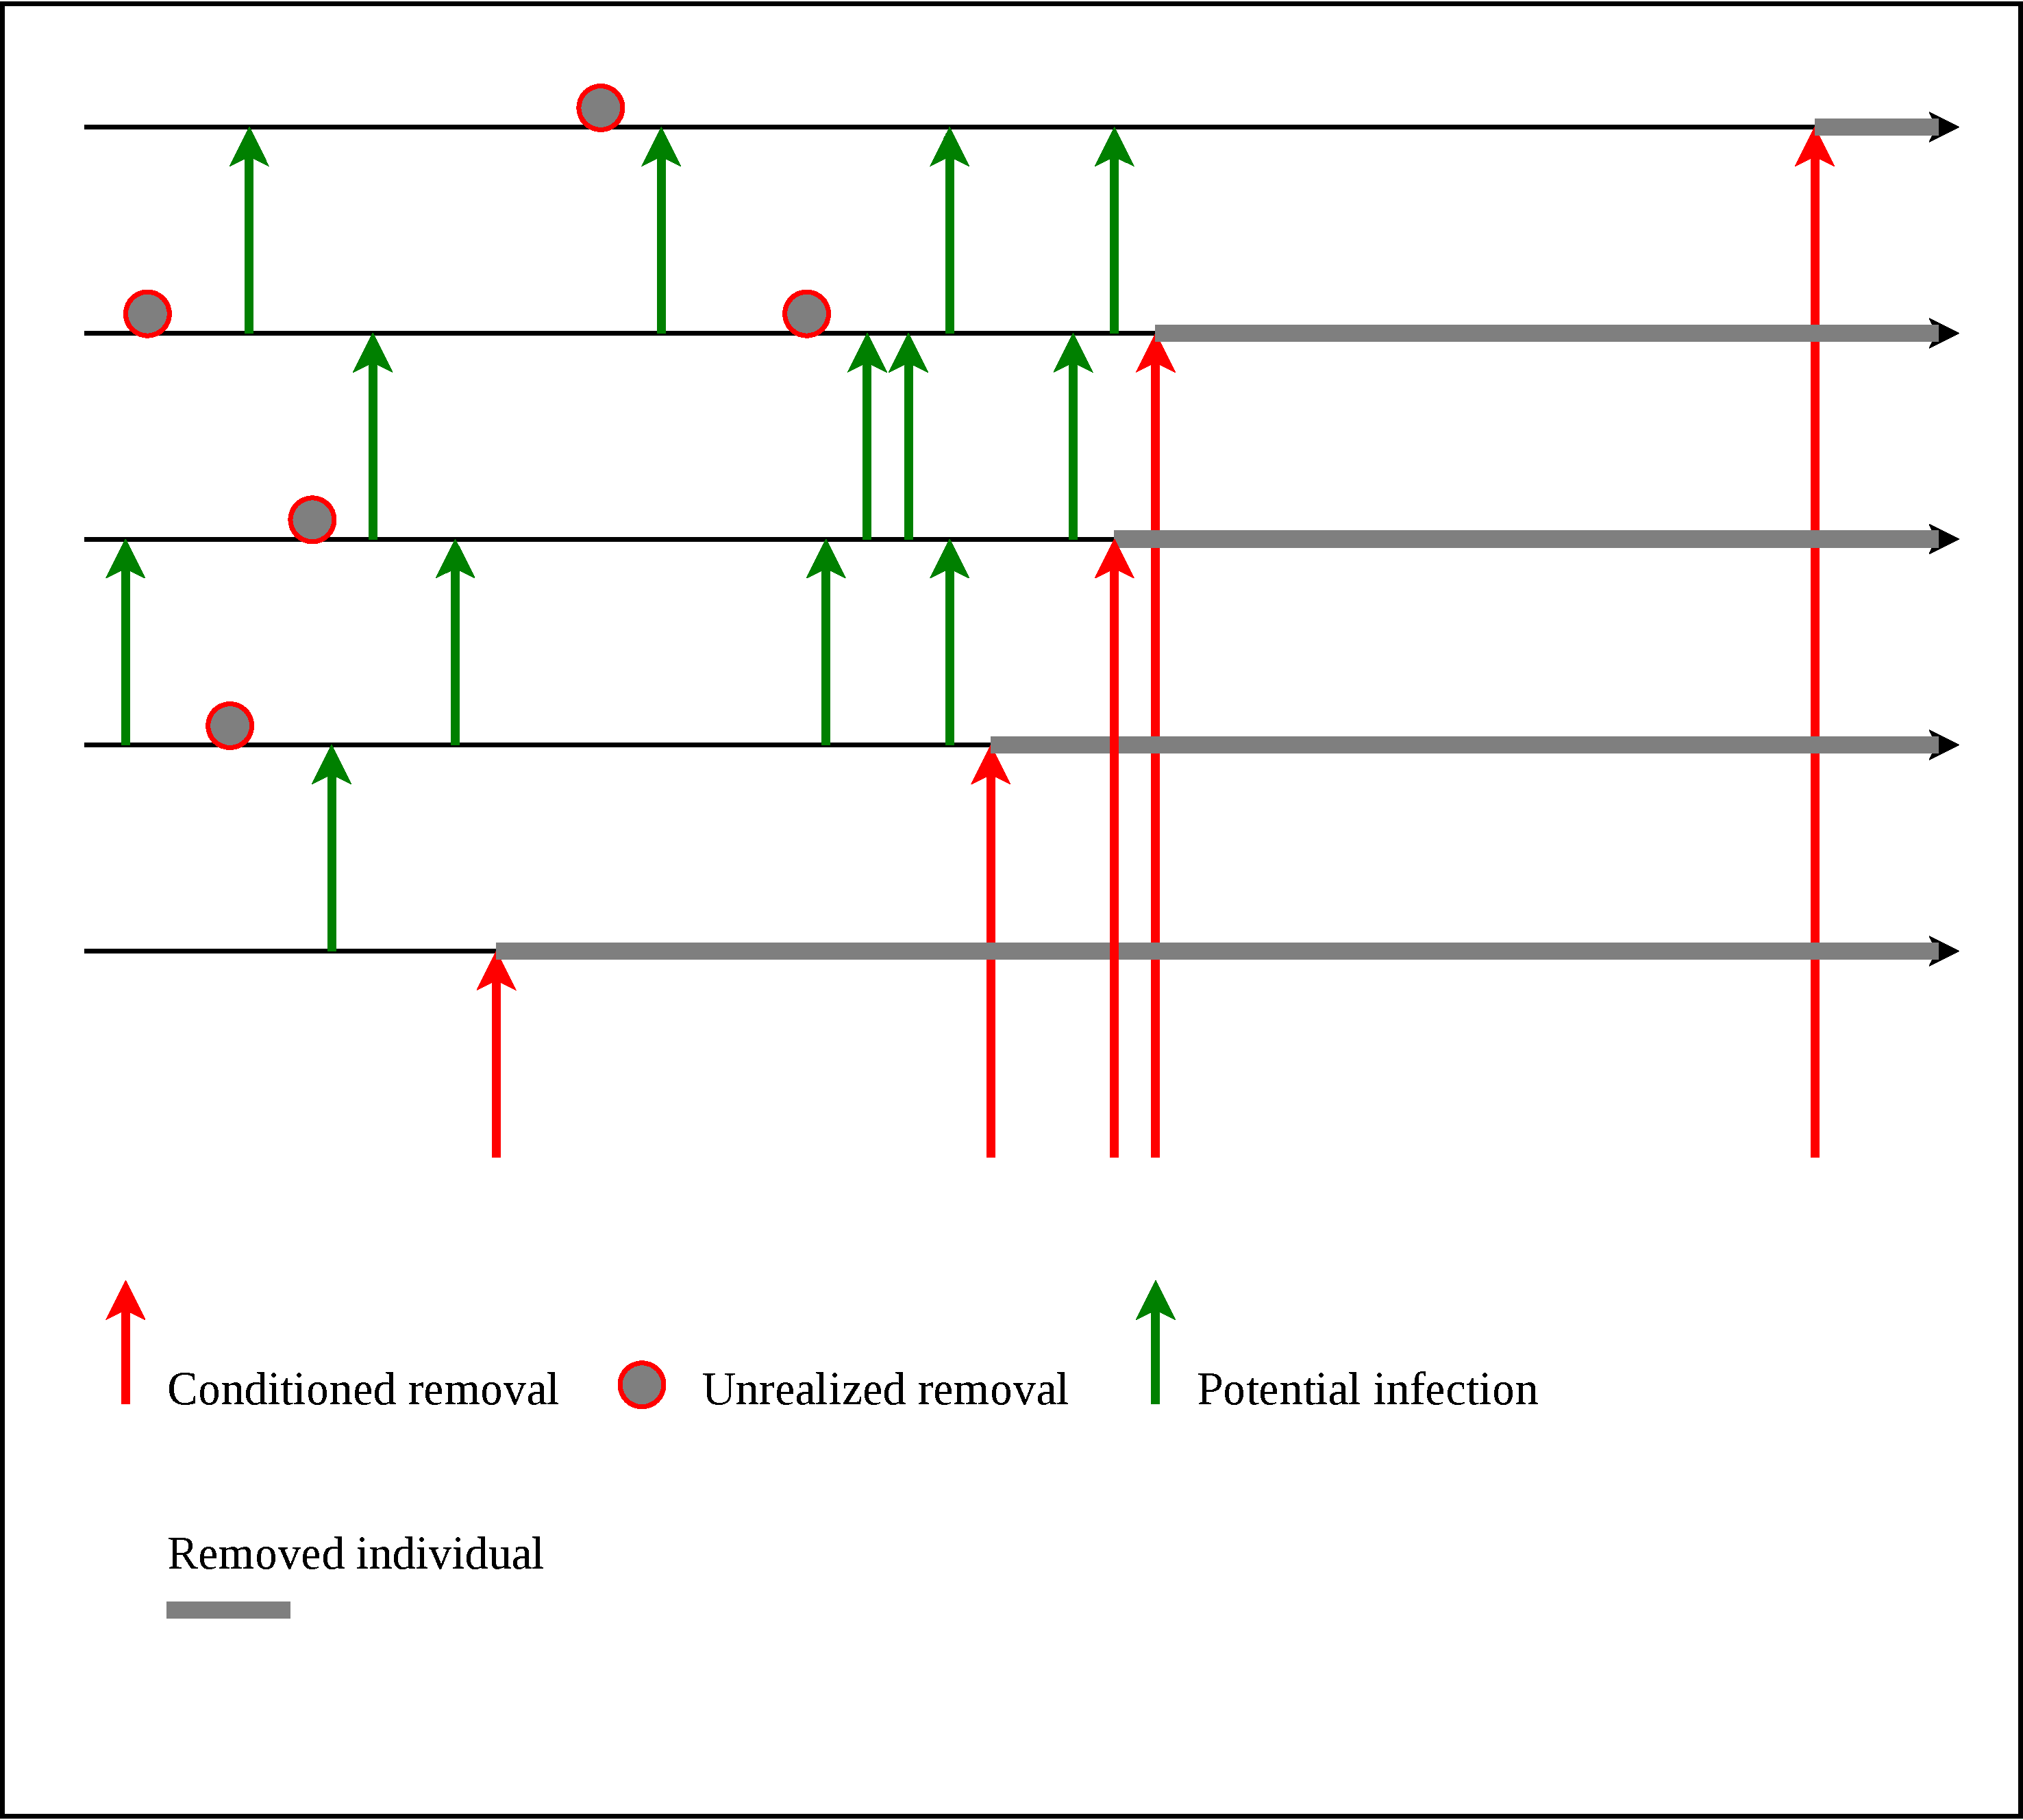
\includegraphics[width=3in]{Timelines1.pdf}
  \caption{Modified graphical representation of \SIR epidemic,
    conditioned on removals.\label{fig:graphical}}
\end{Figure}

 
  \begin{thm}\label{thm:conditioned-SIR-epidemic}
    Suppose \({S}_t\), \({I}_t\), \({R}_t\) measure the susceptibles,
    infectives, and removals arising at time \(\tau\) in stochastic
    equilibrium for the algorithmic-time process given by the modified
    construction described above, but conditioned on the \(n\)
    individuals being removed at removal times
    \(\rho_1<\rho_2<\ldots<\rho_n\).  The process \(({S}, {I}, {R})\),
    viewed in process time, forms an \SIR epidemic conditioned on
    these removals taking place and more generally converges to this
    conditioned \SIR epidemic in distribution as algorithmic time
    tends to infinity..
  \end{thm}
  \begin{proof}[Sketch proof]
    Again we will appeal to detailed (perhaps dynamic) balance.  Note
    that the simulation in algorithmic time of this conditioned \SIR
    epidemic is in this case irreducible, hence allowing the
    convergence result.%
    \NB[WSK2]{Need to explain carefully the irreducibility required
      for Theorem \ref{thm:conditioned-SIR-epidemic}, arising because
      here we count numbers not individuals.}
  \end{proof}
 
 
  % \TBC{Describe the above in terms of epidemic trajectory, boundary
  % of ``no-fly zone'', and trajectory of last viable epidemic.}
  It is helpful to develop a vocabulary describing the boundaries of
  five regions of time-line space, depending implicitly on the
  algorithmic time \(\tau\).  For \(m=1\),\ldots, \(n\), we denote the
  point-set of realized or potential infections on time-line \(m\)
  occurring before removal time \(\rho_m\) by \(\Infections_m\).%
  \NB[WSK2]{Is ``realized'' the opposite of ``potential''? I think the
    use of this terminology needs careful checking: I suspect it is
    used carelessly in the present text.}  Consider the point-set of
  unrealized removals on time-line \(m\) occurring before removal time
  \(\rho_m\); we denote this point-set by \(\Removals_m\).%
  \xNB[WSK2]{Consider avoiding superscripting by referring to
    (process-time) point-sets rather than individual incidents.}
  % Finally we denote by \(\mu_m\) the mark for the realized removal
  % on time-line \(m\) (occurring at process-time \(\rho_m\)).  Note
  % that \(\mu_m\geq m\) is required in order to ensure removal of
  % individual \(m\) at time \(\rho_m\), per conditioning.%
  % \NB[WSK2]{We must have $\mu_m\geq m$ because we are running an
  % \SIR epidemic conditioned so that individual $m$ is removed at
  % time $\mu_m$.}

  Note here that we have suppressed the implicit dependence of
  \(\Infections_m\) and \(\Removals_m\) on \(\tau\).
  % and note also that \(j_m=0\), \(k_m=0\) are both possible; for
  % convenience we write \(\sigma_m^0=0\), \(\rho_m^0=0\).
  Note also that if the \SIR epidemic is to be total (if all \(n\)
  individuals are to be infected) then \(\Infections_m\neq\emptyset\)
  for all \(m<n\).  (It is always true that
  \(\Infections_n=\emptyset\).)  However it is always possible for
  \(\Removals_m=\emptyset\) for some or all \(m\).

  The first region is the \emph{``premature'' zone}.%
  \NB[WSK2]{Do we need specifically to define the ``no-fly'' zone
    boundary?}  This is made up of initial portions of time-lines
  defined by the property, if a time-line point in this region is
  infected then there will result an unconditioned removal.  The
  boundary of the ``premature'' zone is located at process time
  \(\xi_m\) for time-line \(m\), defined inductively by
  % \begin{align}\label{eq:boundary-time}
  %   \xi_n \quad=&\quad \max\left\{\bigcup_{s=1}^n
  %     \Removals_s\cap[0,\rho_s)\right\}\,, &\text{ the last
  %   unrealized
  %   removal on or below time-line }n\,,
  %   \nonumber\\
  %   \xi_m \quad=&\quad \max\left\{\bigcup_{s=1}^m
  %     \Removals_s\right\}
  %   \vee \max\left\{\Infections_m\cap[0,\xi_{m+1}\right)\} &\text{
  %   if
  % }m<n\,.
  % \end{align}
  \begin{align}\label{eq:boundary-time}
    \xi_n \quad=&\quad \max\left\{\Removals_n\cap[0,\rho_n)\right\}\,,
    &\text{ the last unrealized removal on time-line }n\,,
    \nonumber\\
    \xi_m \quad=&\quad \max\left\{\left(\Removals_m \cup
        \Infections_m\right)\cap[0,\xi_{m+1})\right\} &\text{ if }
    m<n\,.
  \end{align}
  (Here and throughout our convention is to set $\max\emptyset :=0$
  and $\min\emptyset := \infty$.) Thus by construction \(\xi_m\) must
  be increasing in \(m\).

  The second region is the \emph{``late'' zone}, whose boundary is
  defined inductively by
  \begin{align}\label{eq:late-boundary}
    \zeta_1 \quad=&\quad
    \min\left\{\Removals_1\cap[0,\rho_1)\right\}\wedge \rho_1\,,
    &\text{ the first removal (unrealized or realized) on time-line
    }1\,,
    \nonumber\\
    \zeta_m \quad=&\quad
    \min\left\{\Removals_m\cap[\zeta_{m-1},\rho_m)\right\}\wedge
    \rho_m &\text{ if } m>1\,.
  \end{align}
  Thus $\zeta_m$ represents the latest possible instant at which
  individual $m+1$ can be infected, if the epidemic is to infect the
  entire population. By construction \(\zeta_m\) must also be
  increasing in $m$, and \(\zeta_n = \rho_n\) since the epidemic is
  conditioned to infect the entire population.  Proposals of potential
  infections with destination in the premature zone, or source in the
  late zone, must be forbidden.  Figure \ref{fig:no-fly} illustrates
  this construction.
  \begin{Figure}
    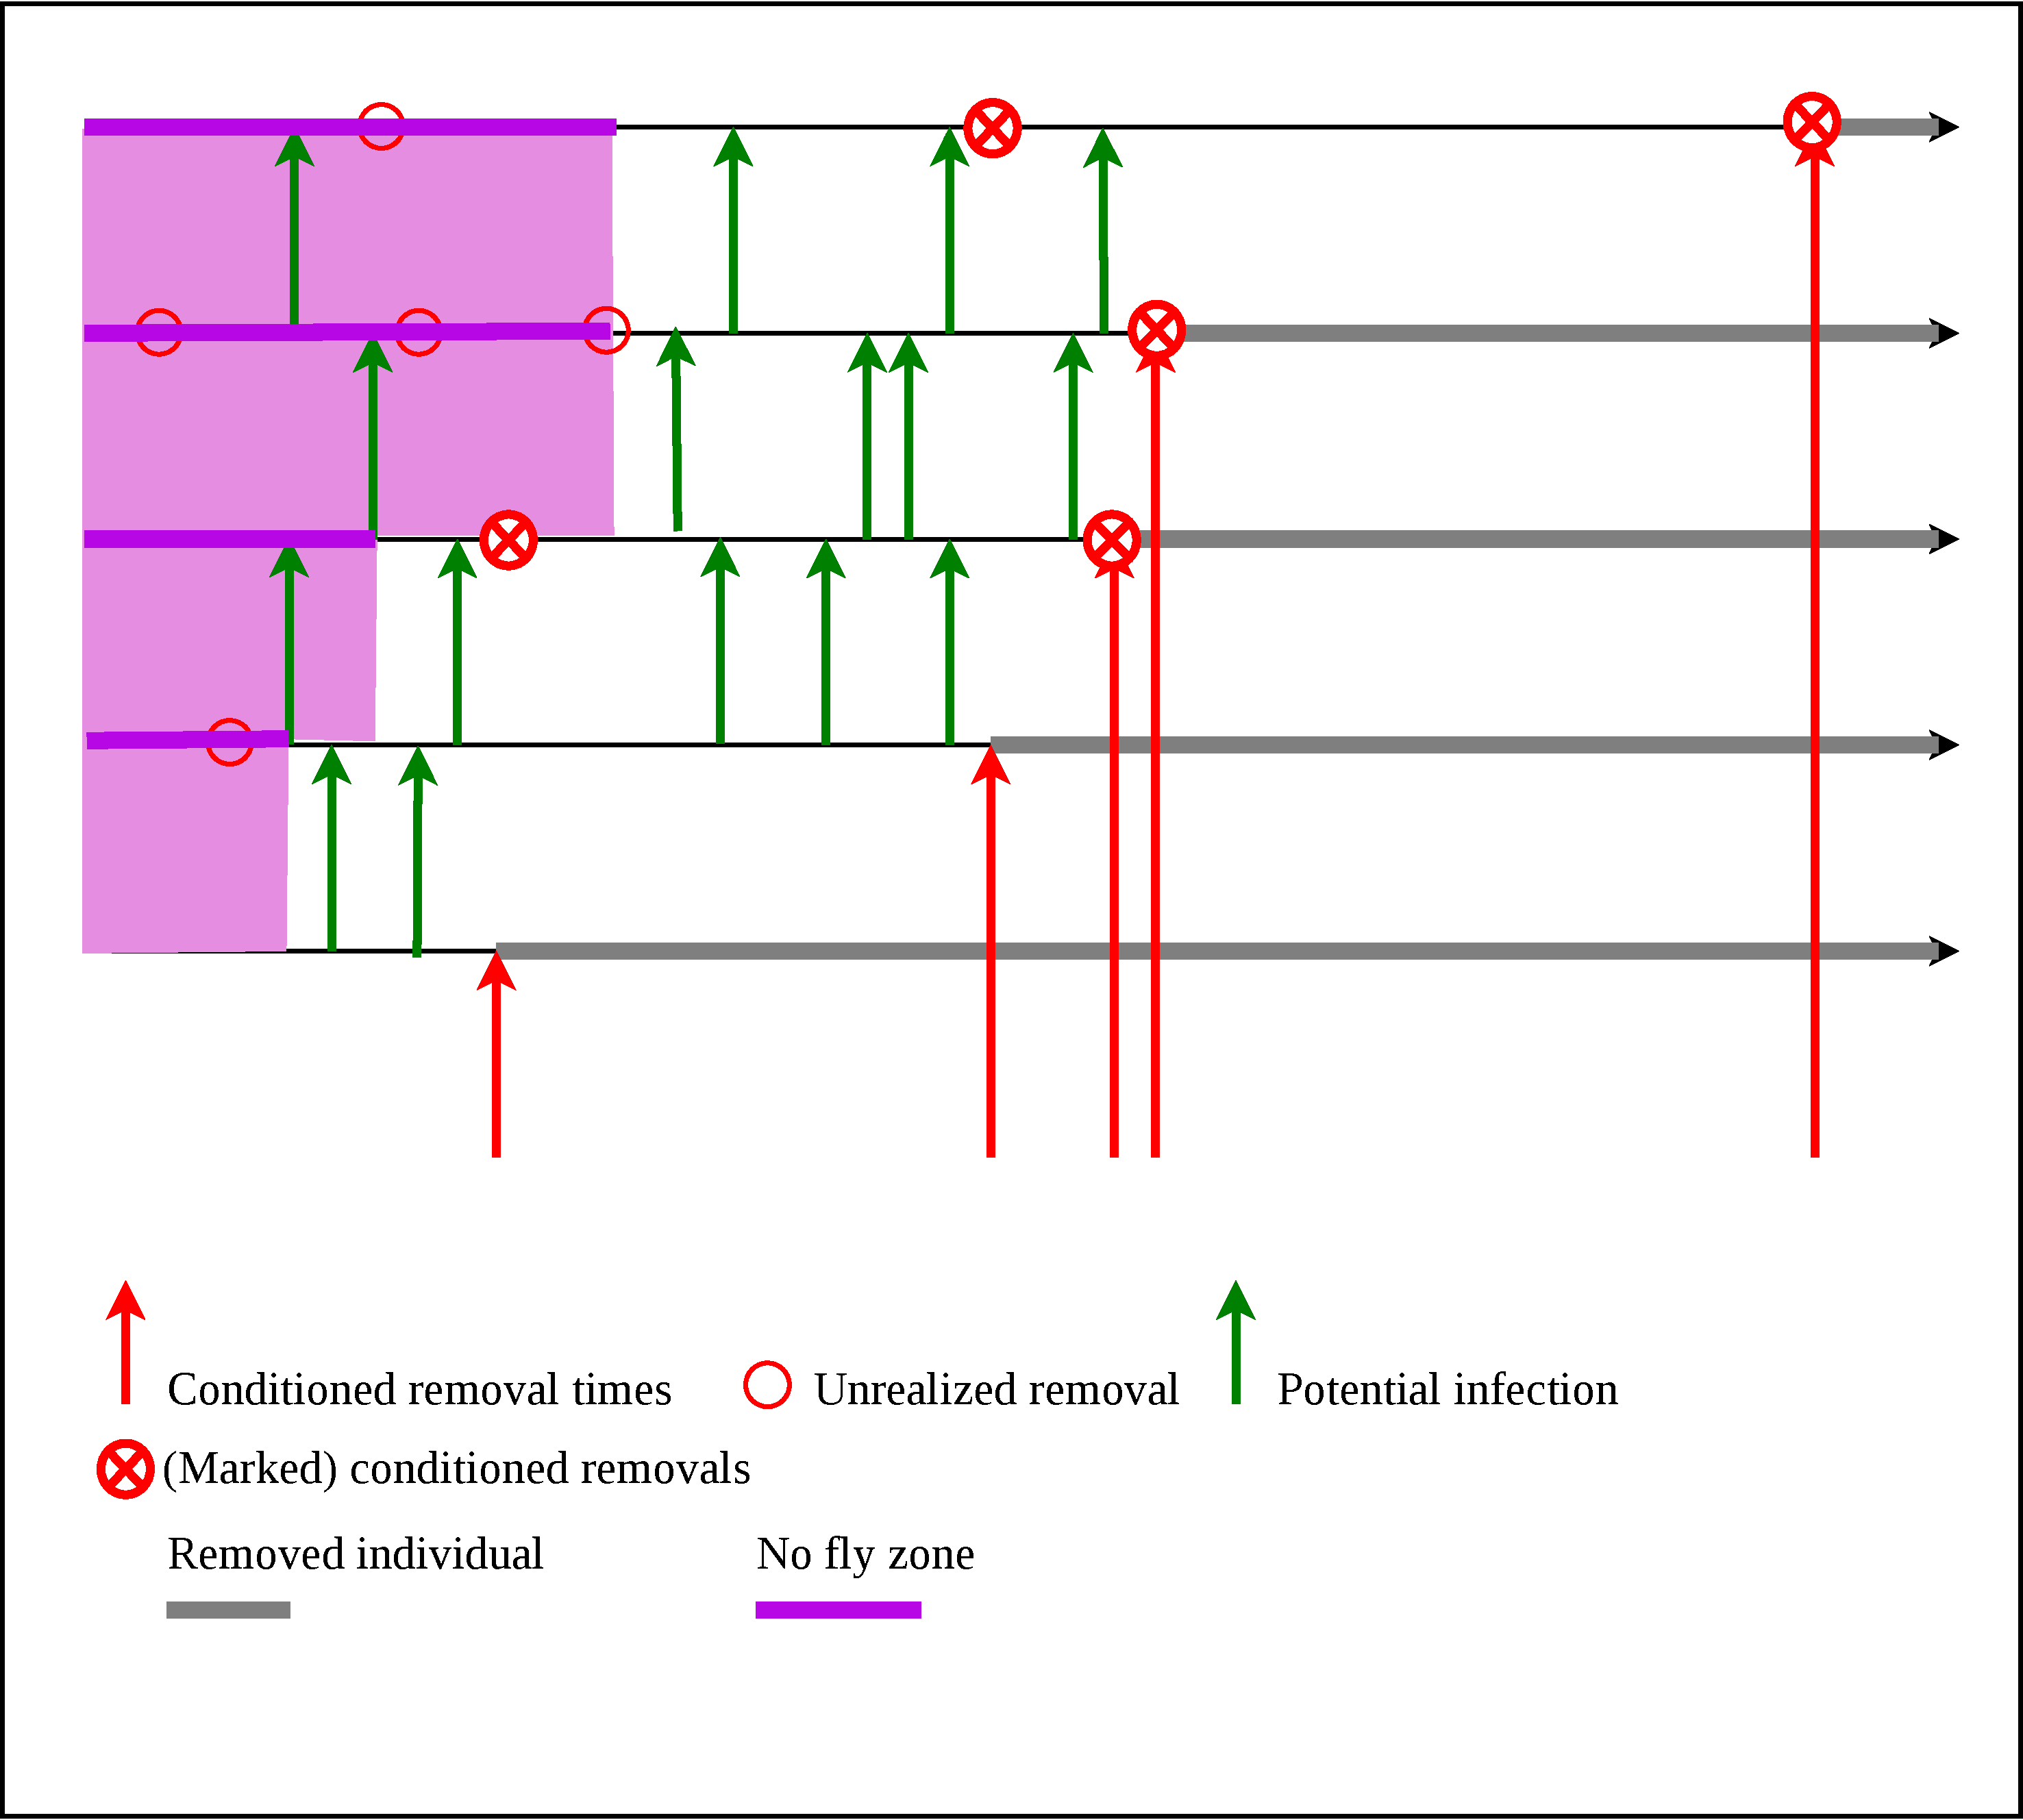
\includegraphics[width=3in]{Timelines2.pdf}
    \caption{``Premature'' and ``late'' zones for this graphical
      representation.\label{fig:no-fly}}
  \end{Figure}
 
  Given the sets \(\Removals\) and \(\Infections\) we can construct
  the ``transmission line'' of the epidemic: this is the counting
  function \(\trans:[0,\rho_n)\to\mathbb{N}\) defined by \(\trans(t) =
  R_t+I_t\). The transmission line is built using those potential
  infections that become realized.  It is located at boundary time
  \(\phi_m\) for time-line \(m\), defined inductively by
  \begin{align}\label{eq:epidemic}
    \phi_m \quad=&\quad 0\,, &\text{ if \(m\leq R_0+I_0=I_0\)}\,,
    \nonumber\\
    \phi_m \quad=&\quad
    \min\left\{\Infections_{m-1}\cap[\phi_{m-1},\rho_{m-1})\right\} &
    \text{otherwise.}
    % \begin{cases}
    %   \infty & \text{ if \(m> R_0+I_0=I_0\) and no potential
    %   infection}
    %   \\
    %   & \text{ from \(m-1\) occurs in
    %   \([\phi_{m-1},{\rho}_{m-1}]\),}
    %   \\
    %   \min\{\sigma_{m-1}^j\;:\; \sigma_{m-1}^j>\phi_{m-1}\} & \text{
    %   otherwise.}
    % \end{cases}
  \end{align}
  Note that \(\phi_m=\infty\) cannot be
  allowed to occur for any \(m\) if we condition on all individuals
  eventually being removed.%
  \xNB[WSK2]{Reformulate (\ref{eq:epidemic}) in a manner similar to
    that of (\ref{eq:last-epidemic}): avoid the case of $\infty$ by
    noting this won't happen under conditioning.}  Necessarily the
  transmission line must avoid the premature and
  late zones, and may not pass through any unrealized removals.
Figure \ref{fig:epidemic}
  illustrates this construction.
  \begin{Figure}
    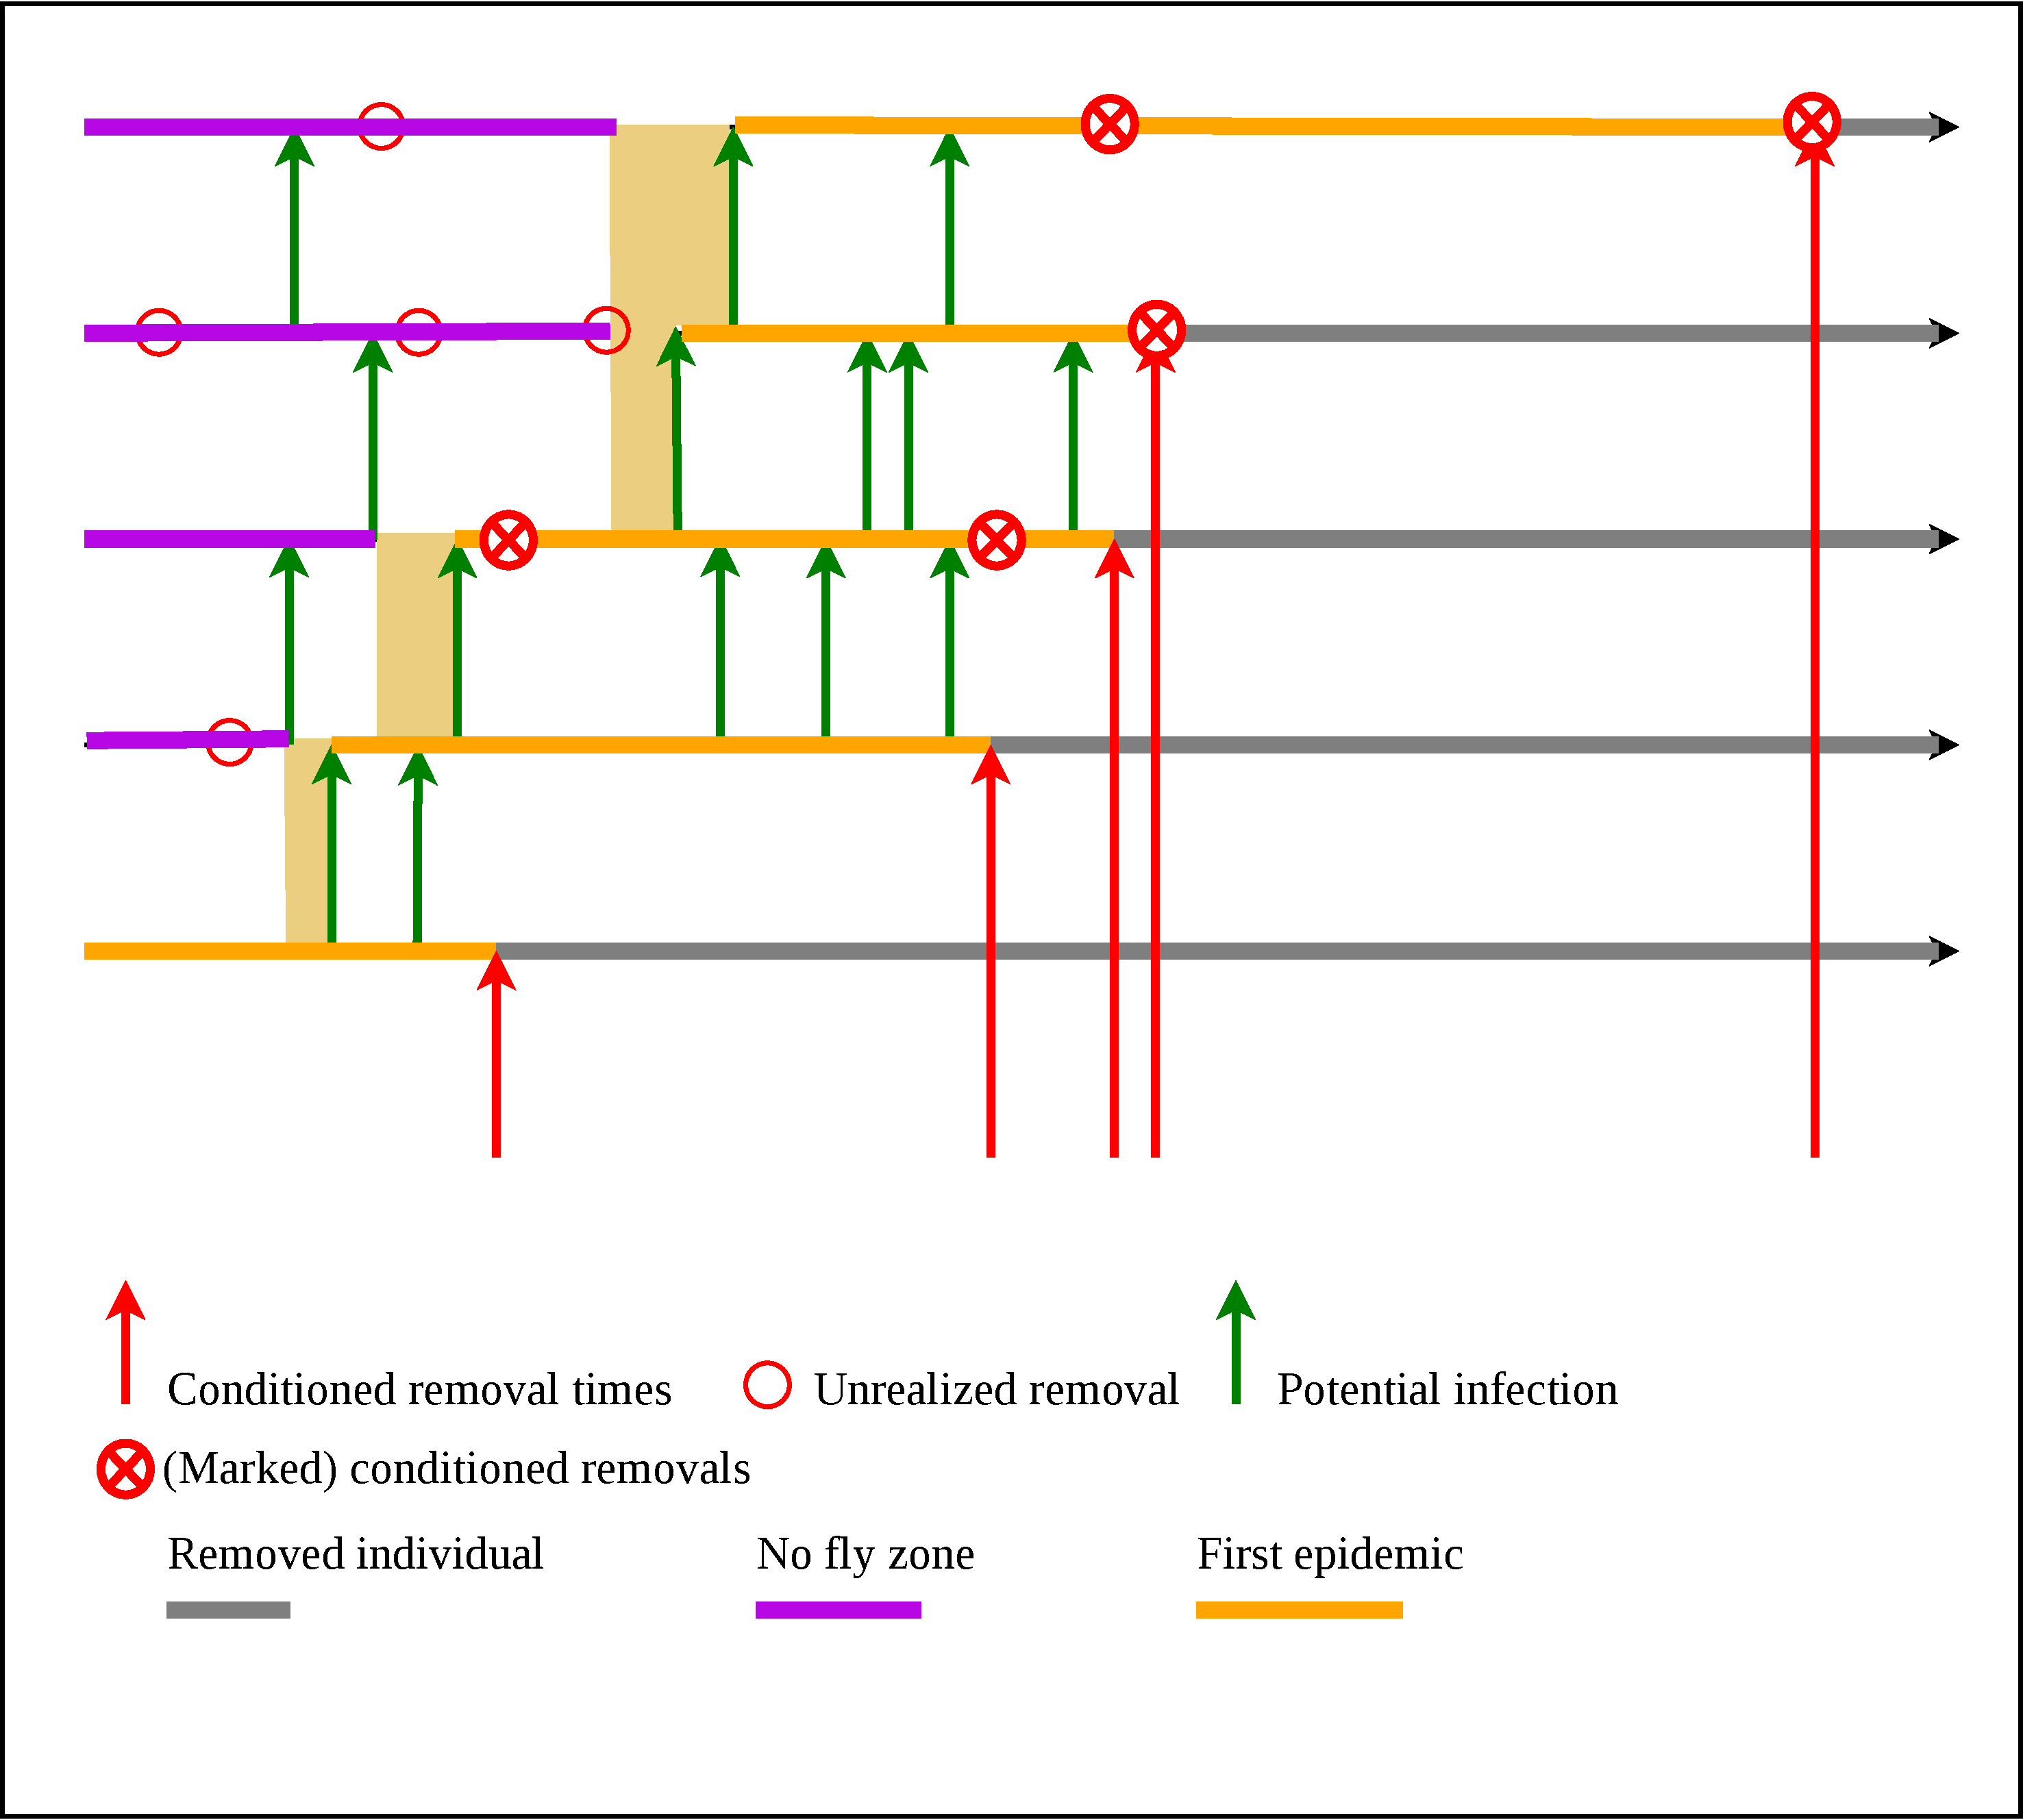
\includegraphics[width=3in]{Timelines3.pdf}
    \caption{Transmission line and last viable epidemic for this graphical
      representation.\label{fig:epidemic}}
  \end{Figure}

  The \emph{last viable epidemic} is the last possible epidemic trajectory
  which avoids unconditioned removals and produces all conditioned
  removals: see Figure \ref{fig:epidemic} for an illustration. %  Together with the epidemic trajectory, it delimits the
  % third region, within which it is possible for an epidemic to proceed
  % to completion.
  It is located at boundary time
  \(\eta_m\) for time-line \(m\), defined inductively by
  \dots\NB[SBC]{This now seems non-trivial to define (working either
    up or down!). Do we need it?}
  % \begin{align}\label{eq:last-epidemic}
  %   \eta_n \quad=&\quad \rho_n\,, \qquad\text{ time of actual removal
  %     for individual \(n\),}
  %   \nonumber\\
  %   % \eta_m \quad=&\quad \max\{\sigma_{m}^j\;:\;
  %   % \sigma_{m}^j<\eta_{m+1} \wedge \rho_m \}
  %   \eta_m \quad=&\quad \max\left\{\Infections_{m}\cap[0,\eta_{m+1}
  %     \wedge \rho_m)\right\} \qquad \text{ if }m<n\,.
  % \end{align}
  % The rationale for the definition of \(\eta_m\) is that the last
  % viable epidemic from time-line \(m\) must certainly infect \(m+1\)
  % prior to the last viable epidemic from time-line \(m+1\), but must
  % also infect \(m+1\) before the conditioned removal of \(m\).  Note
  % that, under the conditioning, the maximum in
  % \eqref{eq:last-epidemic} must be taken over a non-empty set.
  % Figure
  % \ref{fig:last-epidemic} illustrates this construction.
  % \begin{Figure}
  %   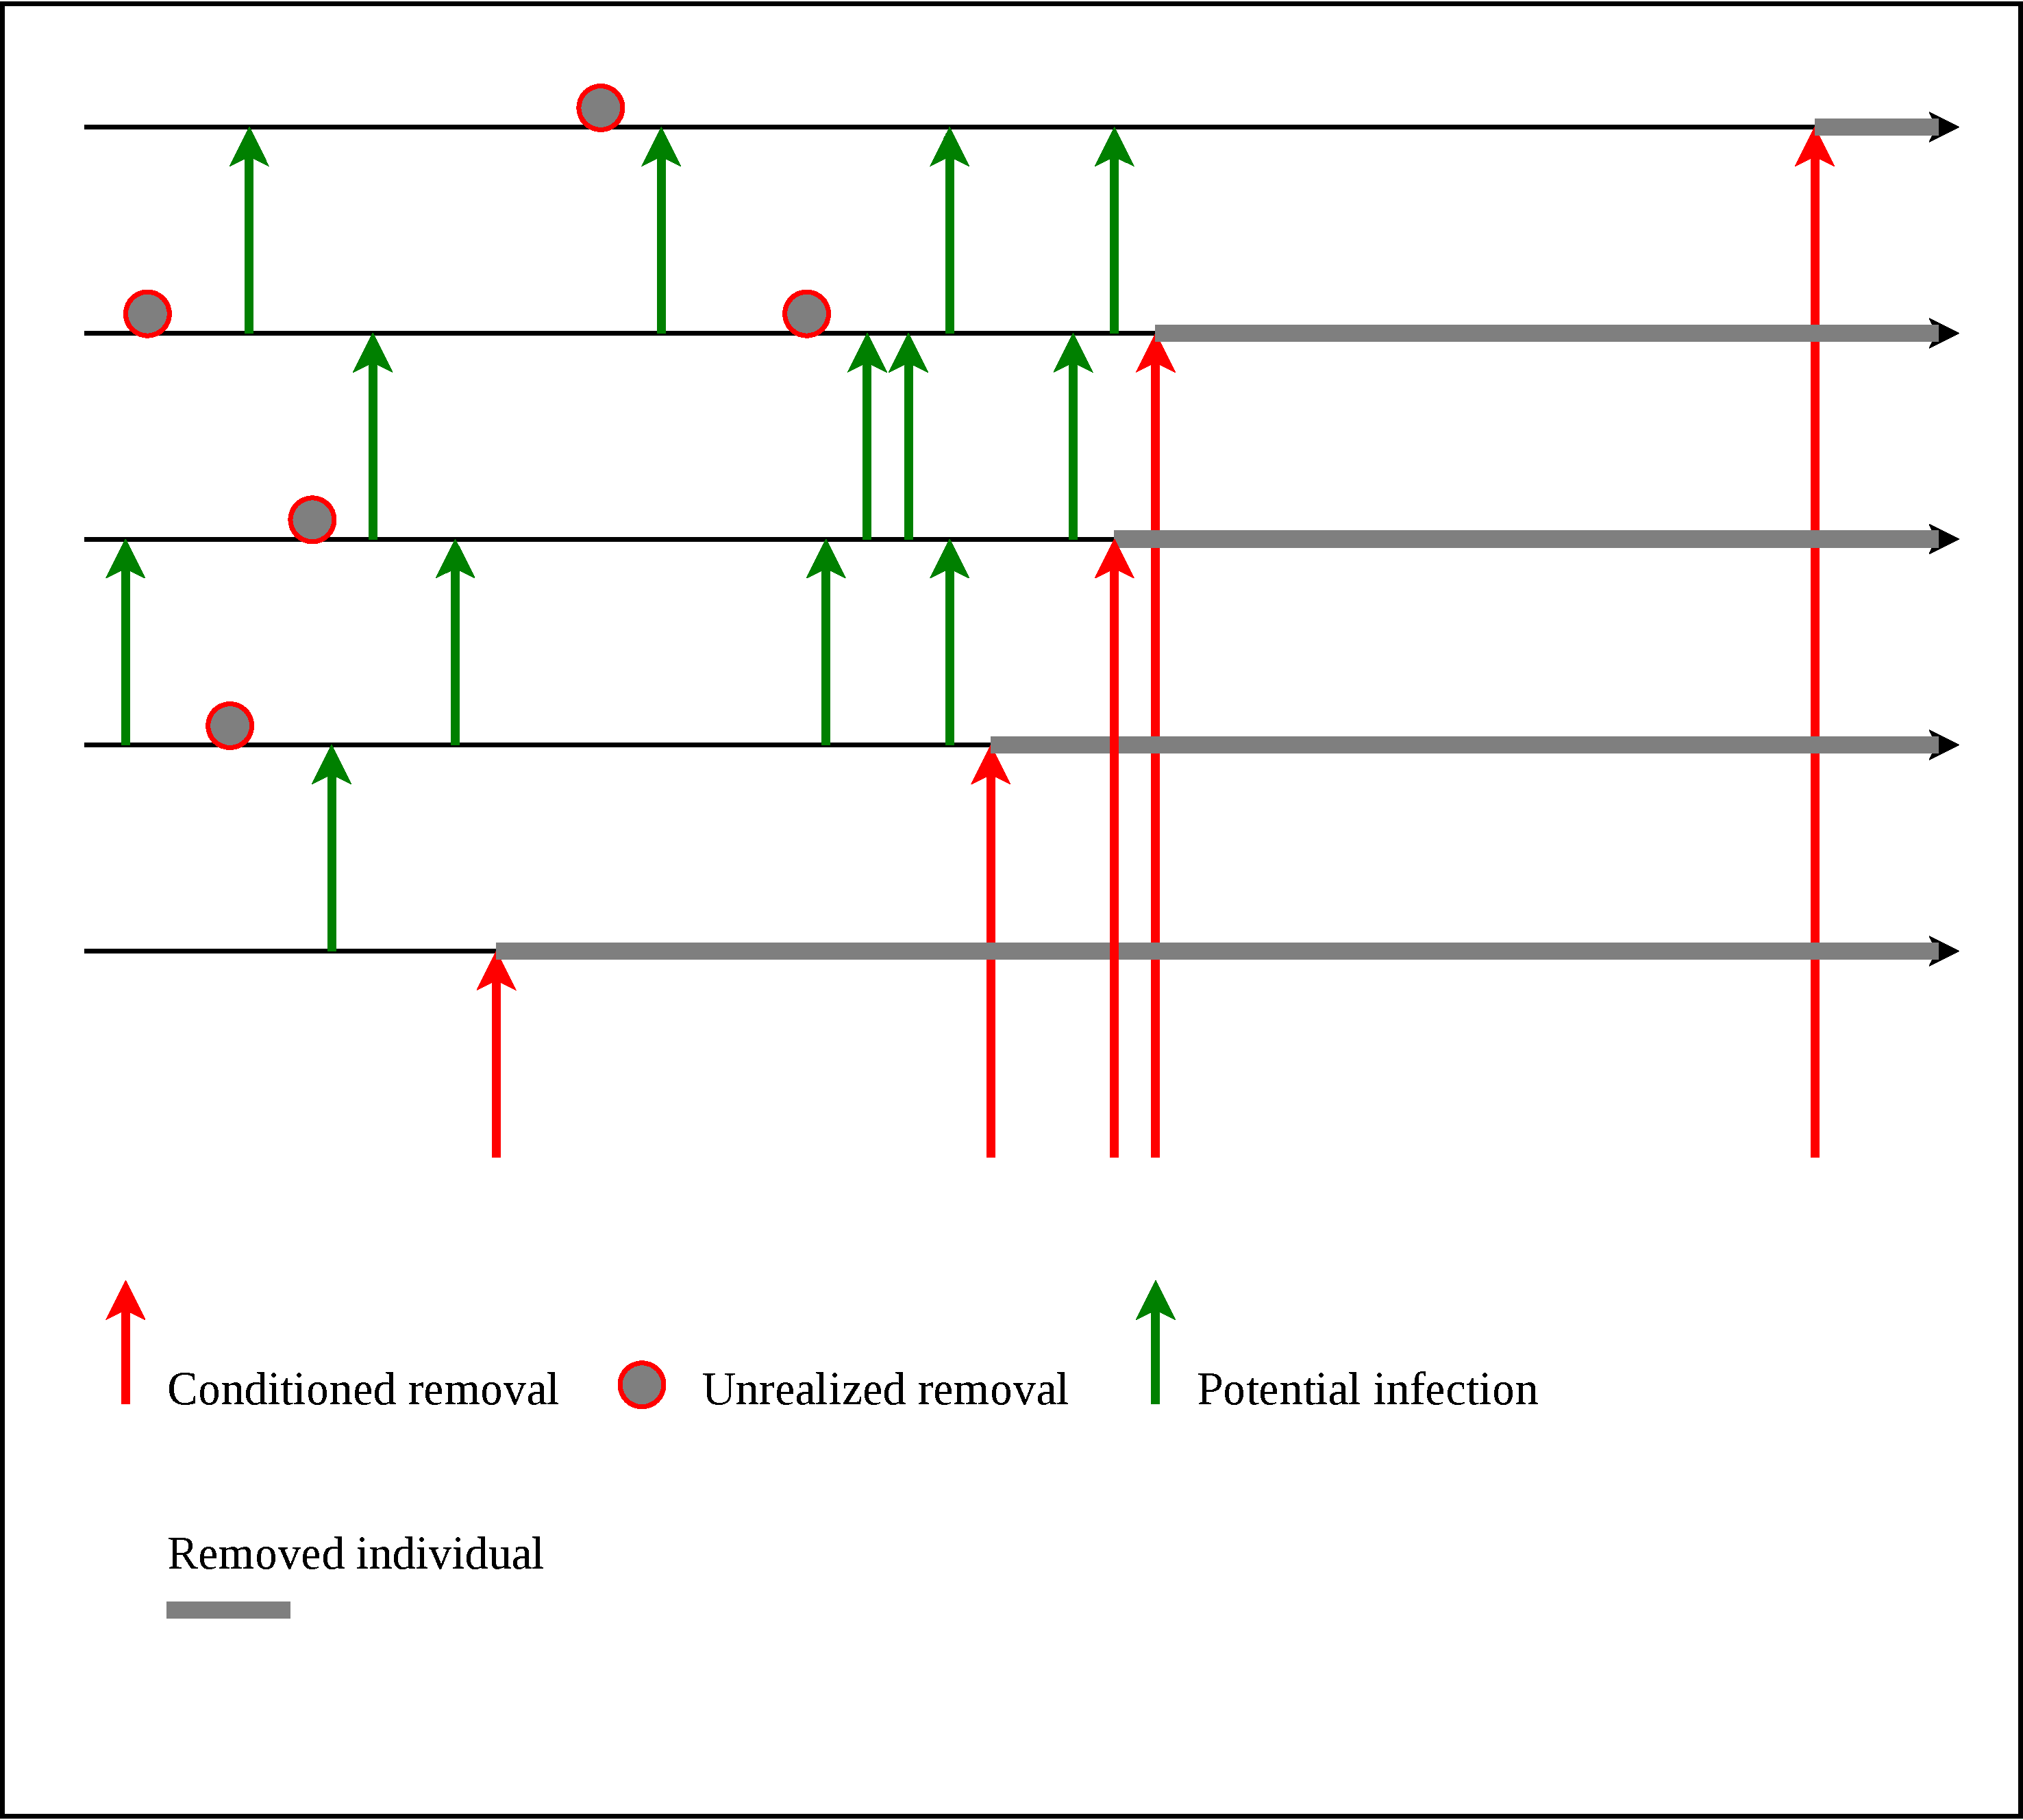
\includegraphics[width=3in]{Timelines1.pdf}
  %   \caption{Third region and last viable epidemic trajectory for this
  %     graphical representation.\label{fig:last-epidemic}}
  % \end{Figure}

  % The fourth region is made up of those parts of infected time-lines
  % from which it would not be possible for an epidemic to proceed to
  % completion, while the fifth region is made up of those parts of
  % time-lines which correspond to individuals removed from the epidemic
  % (Figure \ref{fig:fourth-and-fifth}).  Note that the total of
  % infected portions of time-lines is made up of the union of the third
  % and fourth regions.%
  % \NB[WSK2]{Good names for second, third, fourth and fifth regions?}
  % \begin{Figure}
  %   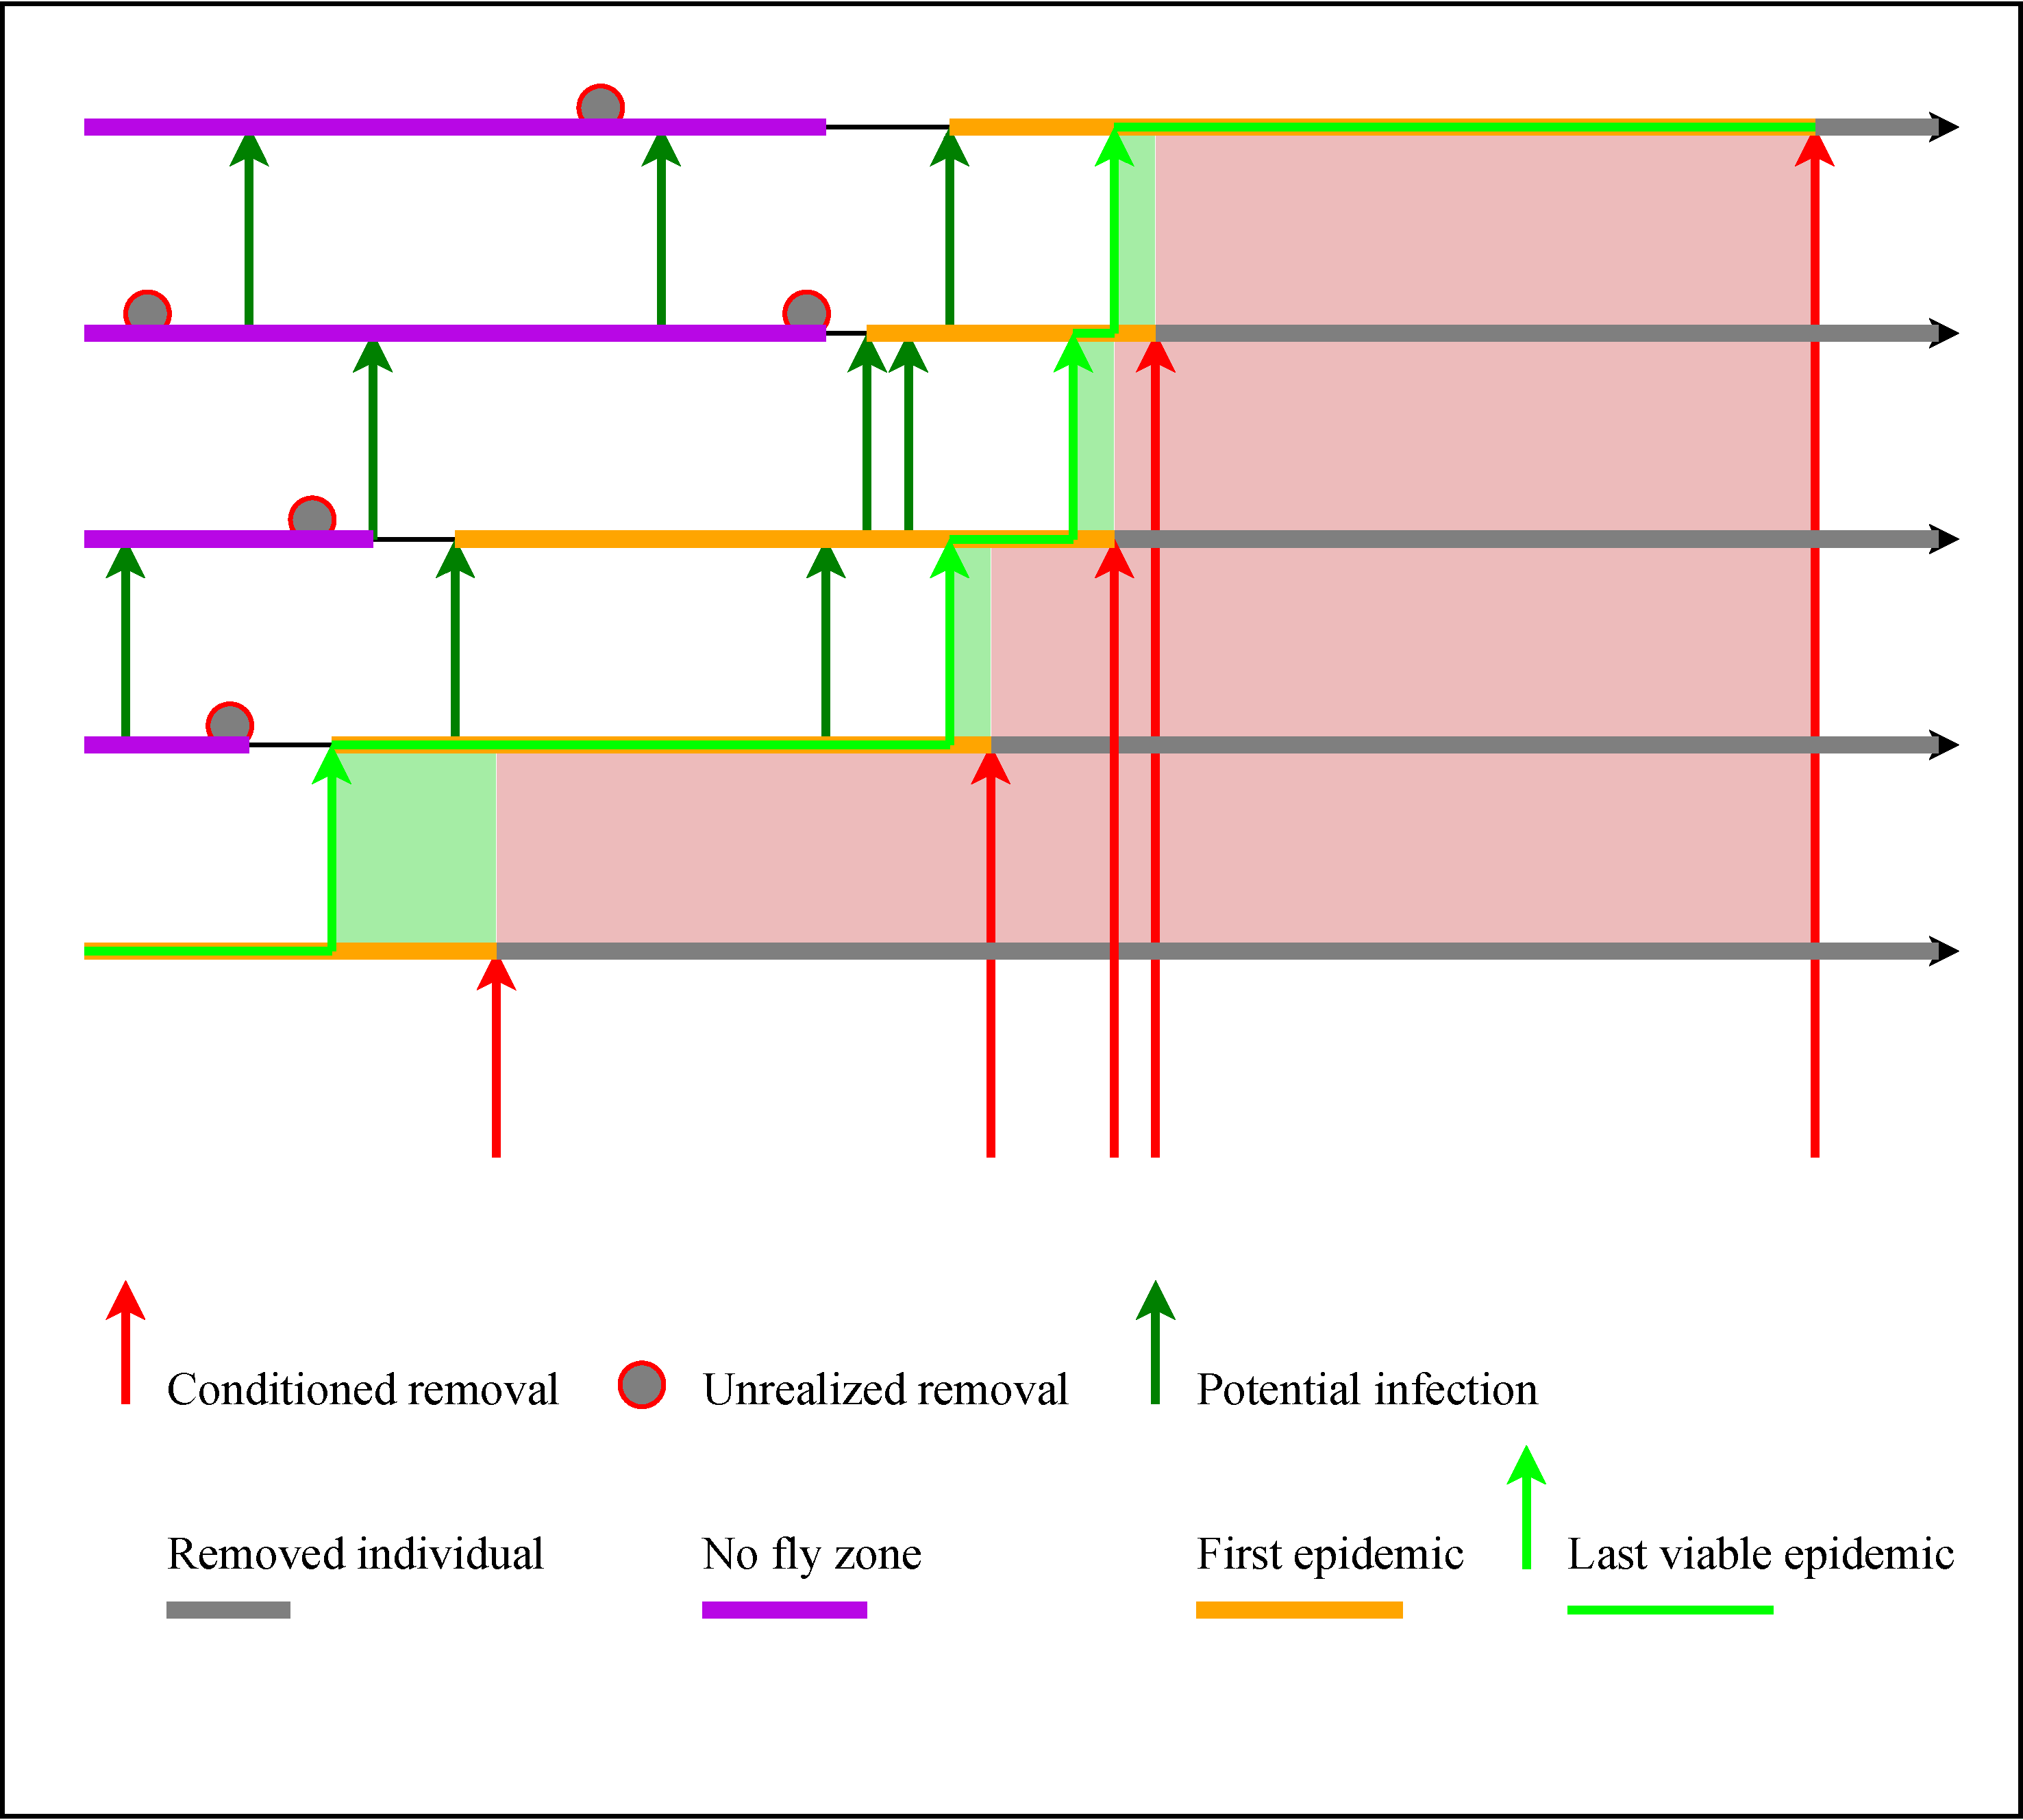
\includegraphics[width=3in]{Timelines5.pdf}
  %   \caption{Fourth and fifth regions for this graphical
  %     representation.\label{fig:fourth-and-fifth}}
  % \end{Figure}

\newpage
  We can now concisely summarize which introductions or deletions of
  potential removals and infections might be refused.  Potential
  removals and infections lying strictly within the fifth region
  (emanating from a removed section of time-line) can be ignored, as
  they do not influence any possible trajectory.  More generally, it
  is always possible to delete an unrealized removal without
  jeopardizing the conditioning; clearly deletion of a realized
  removal must be refused because its deletion would violate the
  conditioning restriction.  Potential removals may only be introduced
  when they are located earlier than the current epidemic trajectory
  on the corresponding time-line; other potential removals would
  become actual infections and so lead to violation of the
  conditioning restriction, and therefore must be refused.
 
  It is always possible to delete a potential infection.  A realized
  infection can be deleted unless it simultaneously forms part of the
  current epidemic trajectory and the current last viable epidemic; if
  it \emph{does} belong to both these epidemics then it may not be
  deleted without violating the conditioning, and therefore its
  deletion must be refused.  In other words, realized infections
  currently belonging simultaneously to first and last epidemics must
  always be perpetuated, and these are the only infections subject to
  perpetuation.  Potential infections can be introduced unless they
  would currently connect the epidemic trajectory to the ``no-fly''
  zone.  So potential infections can be introduced (whether or not
  they become actual) unless the introduction bridges the gap between
  epidemic and ``no-fly'' zone.
 
  We now formalize a number of these observations in the form of
  lemmas, which should be useful when establishing monotonicity of the
  epidemic trajectory.%
  \NB[WSK2]{Terminology: ``earlier'' and ``later'' often refer to the
    time-line ordering, as in ``a potential infection earlier than the
    epidemic''.}
 
 \begin{lem}\label{lem:infect1}
   Potential infections with source and destination no earlier than
   the epidemic trajectory will always be realized (if we exclude
   cases in which source lies in the removal region).
 \end{lem}
 \begin{proof}
   \textbf{(to be completed)}
 \end{proof}

 \begin{lem}\label{lem:infect2}
   Potential infections with source strictly earlier than the epidemic
   trajectory and destination lying within the ``no-fly'' zone will
   extend the ``no-fly'' zone.
 \end{lem}
 \begin{proof}
   \textbf{(to be completed)}
 \end{proof}

 \begin{lem}\label{lem:infect3}
   Current infections are perpetuated exactly when they simultaneously
   form part of the current epidemic trajectory and the current last
   viable epidemic.  Moreover at any fixed algorithmic time \(\tau\)
   there can be at most one perpetuated infection on each time-line.
 \end{lem}
 \begin{proof}
   \textbf{(to be completed)}
 \end{proof}

  \begin{lem}\label{lem:removal1}
    Consider the phase of algorithmic time \([2(m-1)T, (2m-1)T)\)
    during which potential removals are introduced.  This can be
    implemented very directly as follows:
    \begin{enumerate}
    \item remove all current potential removals;
    \item for each time-line \(m\), introduce new potential removals
      according to a Poisson process of time-varying intensity
      \(\beta(m-R_t)\) over the range \([0,\phi_m]\), where \(\phi_m\)
      is (as above) when the time-line \(m\) currently becomes
      infected.
    \end{enumerate}
  \end{lem}
  \begin{proof}
    \textbf{(to be completed)}
  \end{proof}

 
  % \begin{thm}\label{thm:conditioning}
  %   If the dynamic process in algorithmic time is restricted so as
  %   to stay within the subset of configuration space corresponding
  %   to conditioned removals, then the restricted process has the
  %   conditioned \SIR epidemic as equilibrium distribution.
  % \end{thm}
  % \begin{proof}[Sketch proof]
  %   Verify detailed (perhaps dynamic) balance is satisfied.%
  %   \NB[WSK1]{Need to complete the statement and proof of Theorem
  %   \ref{thm:conditioning}.}
  % \end{proof}

 
  % =========================================
 \section{Monotonicity and \CFTP}\label{sec:cftp}
\TBC{
Simulation 
\\
 Discover monotonicity structure to allow for \CFTP constructions.
\\
To make sure we have a secure understanding of this, we should consider how to build a robust simulation programme for the algorithmic time evolution. 
In particular, we need to check reversibility and conditioning arguments, as well as evaluating the possibility of monotonicity structures.  
\begin{itemize}
 \item Monotonicity structures;
 \item Proofs;
 \item Sandwiching;
 \item \CFTP algorithm.
\end{itemize}
}
%
\TBC{I believe all we need to prove here is the following:
\\
Suppose we have two separate conditioned \SIR epidemics (epidemics (I) and (II)) driven by the same sequences of potential removals and potential infections as above.
Suppose further that at some algorithmic time \(\tau_0=2mT\) for some integer \(m\) it is the case that
\begin{itemize}
 \item the ``no-fly'' zone for epidemic (I) is contained in that of epidemic (II);
 \item the epidemic trajectory for epidemic (I) is never later than that for epidemic (II);
 \item the last viable epidemic for epidemic (I) is never later than that for epidemic (II);
 \item (Consequently, on each time-line containing perpetuated incidents for both epidemics, the perpetuated incident for epidemic (I) is never later than that for epidemic (II);)
 \item the set of un-perpetuated realized infection incidents for epidemic (I) contains the set of un-perpetuated realized infection incidents for epidemic (II);
 \item the set of un-realized infection incidents for epidemic (I) is contained in the set of un-realized infection incidents for epidemic (II).
\end{itemize}
Then an inductive argument (inductive on the sequence of proposed incidents in the above construction)
maintains this ordering for all algorithmic times \(\tau\geq\tau_0\).
}
\TBC{I believe that the full \CFTP construction follows quickly from this.}

% =========================================   
 \section{Examples}\label{sec:examples}
\TBC{Simulation output. Applications to a real dataset?}
%

% =========================================   
 \section{Conclusion}\label{sec:conclusion}
\TBC{
\begin{enumerate}
 \item Perfect simulation to include inference about parameters \(\alpha\) and \(\beta\)? (Omnithermal simulation?)
 \item More general compartment models?
 \item Moving from Poisson processes to shifted renewal processes?
\end{enumerate}
}
%

% =========================================   
%   \scriptsize \input hyperbib
%   \label{sec:bibliography}
   \bibliographystyle{chicago}
   \bibliography{PerfectEpidemics}

\appendix
\twocolumn
\pagenumbering{alph}
\setcounter{page}{1}

\TrackingPostamble

\end{document}
